\chapter{Introduction}
\label{ch:introduction}
Robots are becoming more and more present in the day-to-day life helping humans
in different scenarios:
\begin{itemize}
  \item Industrial: this is possibly the aspect in which automated
    machines have had the most successful applications. Indeed, the 4.0
    industrial revolution meant for many workers the beginning of interaction 
    with the machines present in the factories \cite{industry4_0}, showing great
    results~\cite{coordinationInWarehouse}. One of the most known examples of 
    robotics applied to the industry is Spot from Boston Dynamics, which not 
    only can freely move in the environment and record it with its cameras, but
    can also find possible problems and predict which components will need
    maintenance when integrated with sensors~\cite{bostonDynamics}. This is but
    an example of how robotics can be applied to the industrial environment.
    Indeed, robotics proves to enhance and solve more and more easily logistics
    manufacturing problems allowing for a better use of the industrial
    space~\cite{industry4_0_1}.
  \item Healthcare: for the last decade, robots have started being used with
    great profits in this sector. For example, they have been successfully used
    in precise surgical procedures to help surgeons reaching anatomical
    compartments and doing operations that would otherwise be impossible
    \cite{surgicalRobot}. Also, robotics has been applied to help elderly and
    impaired people move more freely, besides being used to assist during
    rehabilitation~\cite{friWalker}.
  \item Search and rescue: robots have been successfully utilized also in
    search and rescue missions in challenging environments
    \cite{searchRescueDrones}, where the situation may endanger also the
    rescuers. 
  \item Office robots: robots can be used to help in the day-to-day life of an 
    office allowing affairs to sped up and simplifying the general 
    workday~\cite{cobots}.
\end{itemize}
In the majority of these situations, there are multiple robots that need to
cooperate with each other in order to complete one o multiple tasks in the most
efficient way. Moreover, having the robots follow human-aware trajectories, 
dramatically increases the reliability and safety of the environment, while yet
keeping the benefits of using robotics in the scenario.
\begin{figure}[htpb]
  \centering
  \includegraphics[width=0.32\textwidth]{warehouse}
  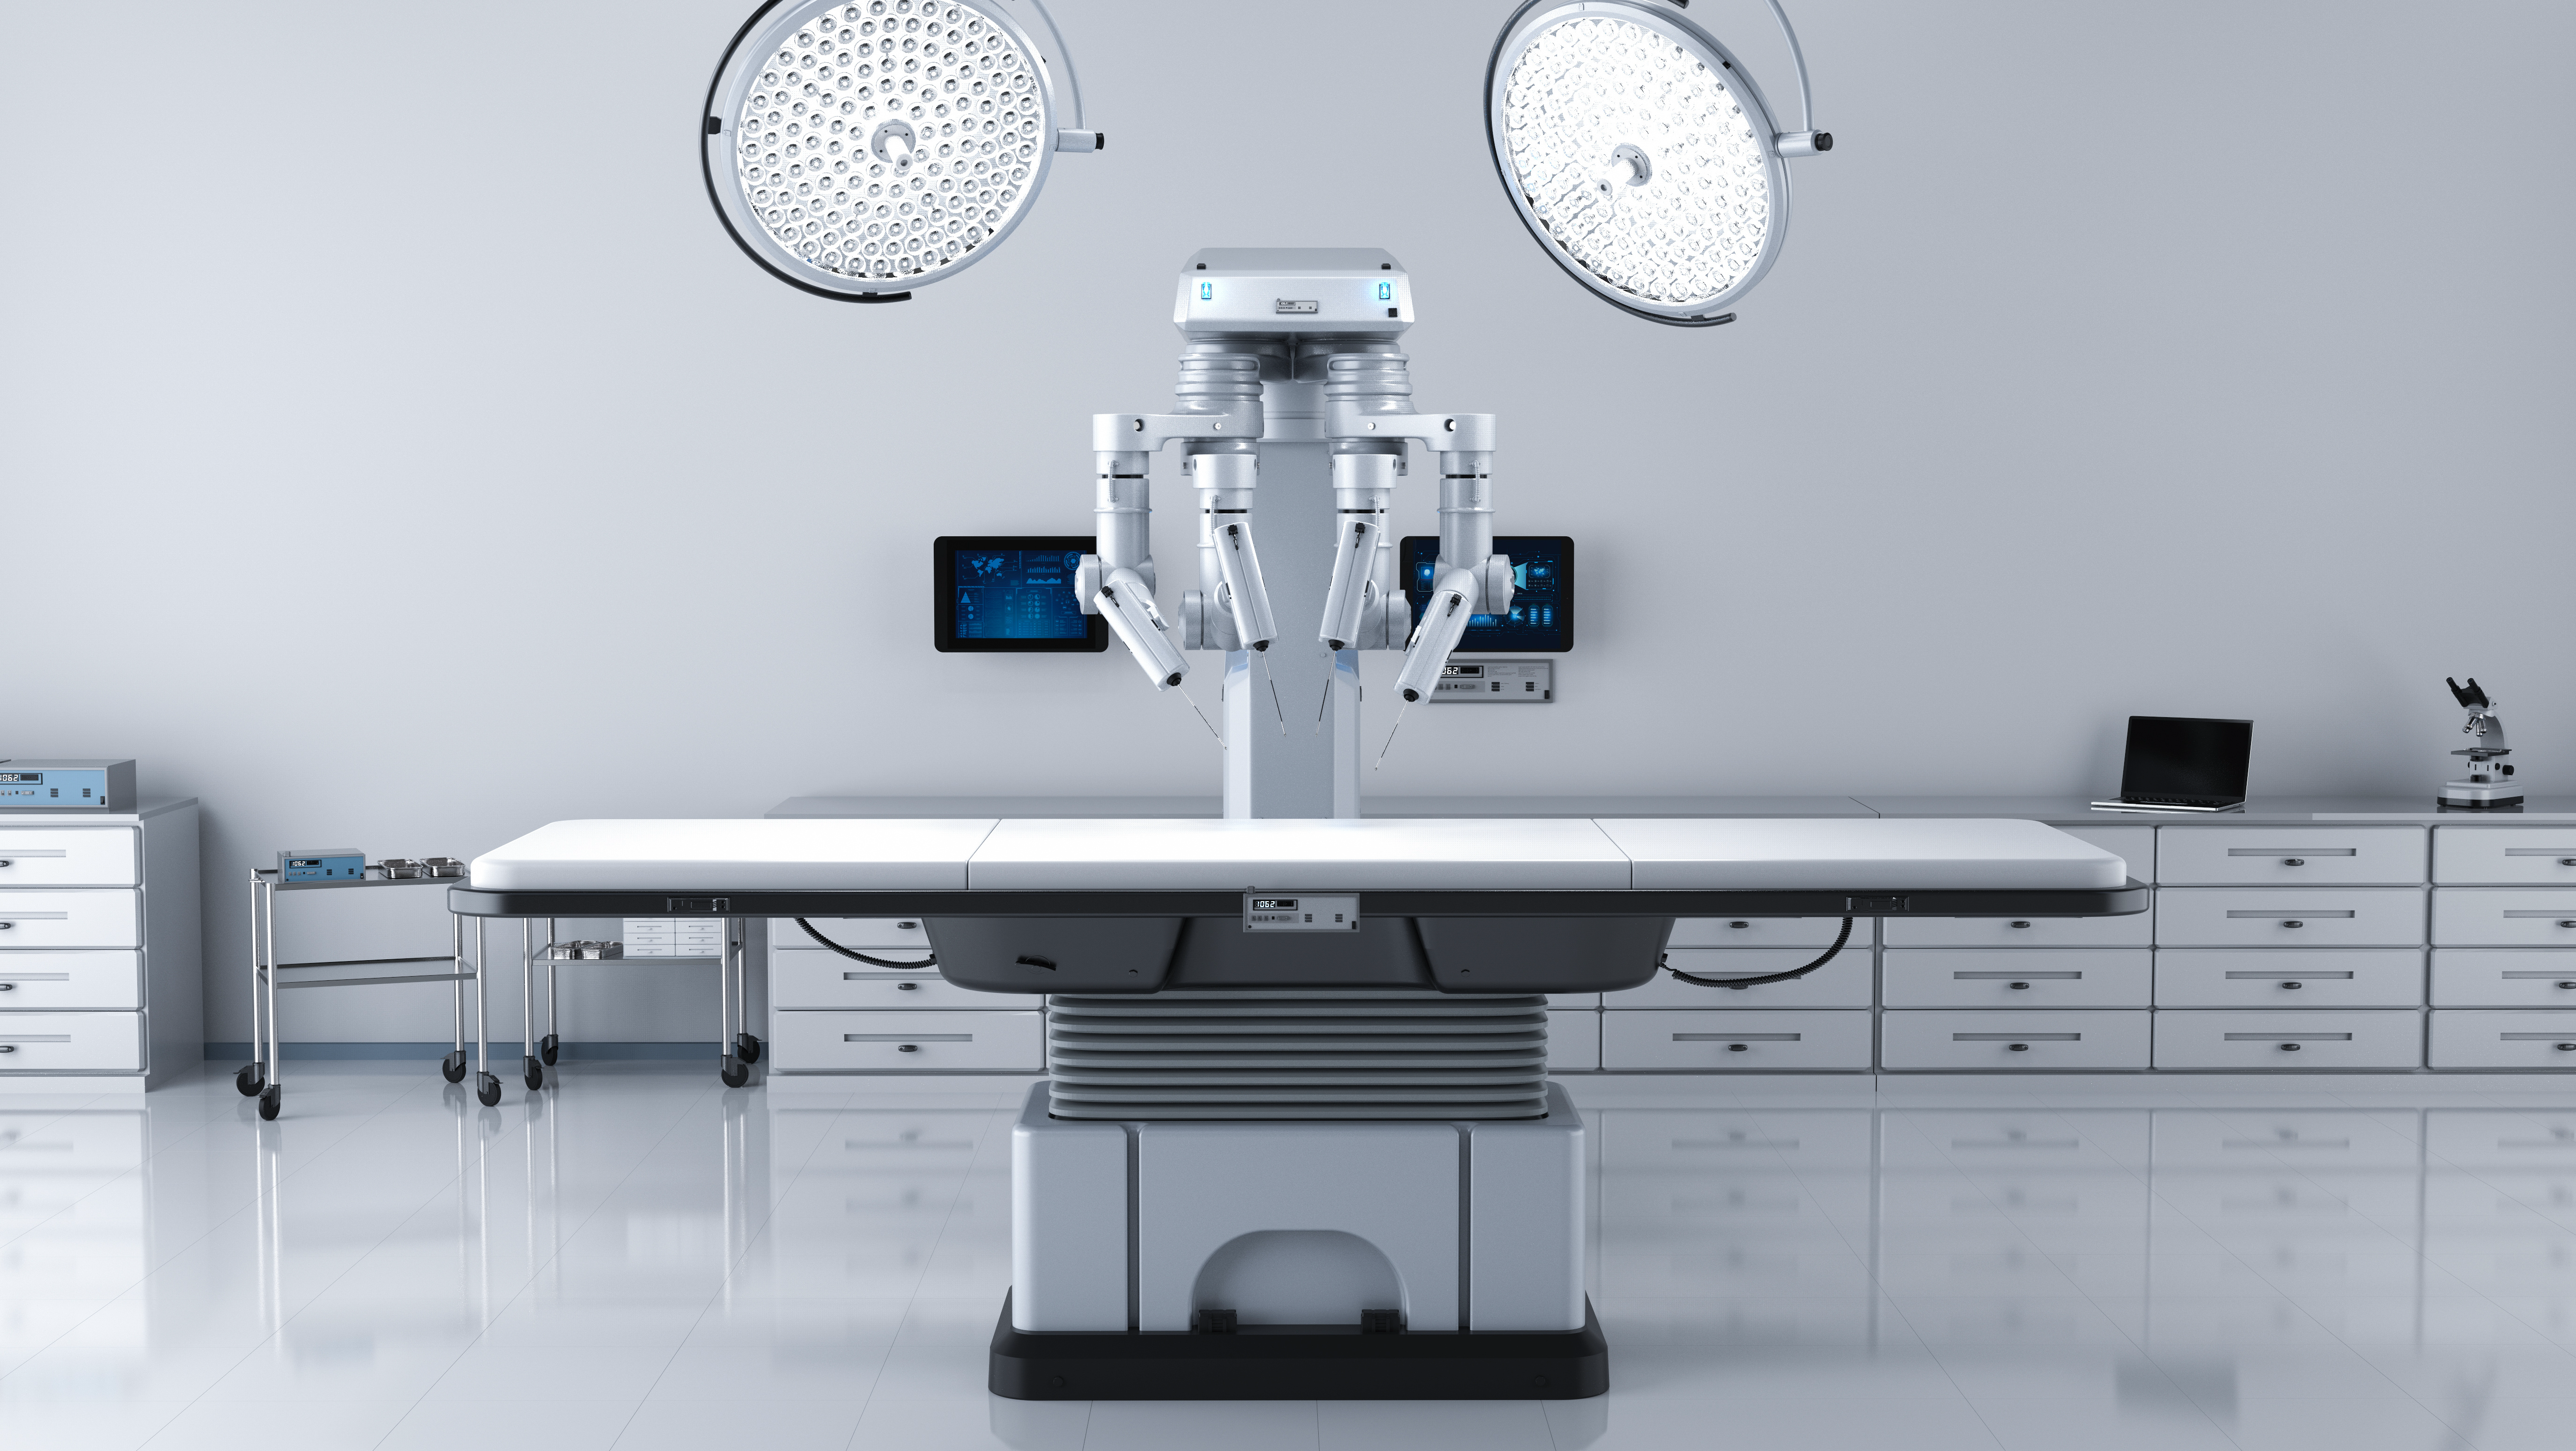
\includegraphics[width=0.32\textwidth]{surgeon1}
  \includegraphics[width=0.32\textwidth]{rescue}
  \caption{Robots can be employed in a different number of scenarios to help
  humans, from the movement of heavy packages in warehouses, to the precision
  of surgery, and also to help search and rescue in remote environments.}
  \label{fig:robot_examples}
\end{figure}
%
%
%
\import{./}{1-SafeMotionPlanning}
\import{./}{2-SAPF}
\import{./}{3-MAPF}
